\documentclass[10pt,twocolumn]{article}

\usepackage{times}
\usepackage{fullpage}

\usepackage{booktabs}  % for \midrule
%\usepackage{subfigure}
\usepackage{balance}
\usepackage{graphicx}
\usepackage{xspace}
%\usepackage{pslatex}
%\usepackage{pifont}
%\usepackage{multirow}
%\usepackage{array}
%\usepackage{booktabs}
%\usepackage{cite}
\usepackage{url}
%\usepackage{cancel}
\usepackage{color,colortbl}
%\usepackage{microtype}
%\usepackage{textcomp}% http://ctan.org/pkg/textcomp
\usepackage{tabularx}
\usepackage{framed}
\usepackage[]{algorithm2e}
\SetAlFnt{\small}
\SetAlCapFnt{\small}
\usepackage{algorithmic}

\usepackage{listings}
%\usepackage{scrextend}
%\usepackage{mathtools}
\usepackage{pbox}

\let\labelindent\relax
\usepackage{enumitem}

\usepackage{tikz}
\usetikzlibrary{arrows,automata}
\usetikzlibrary{calc,positioning}
\usepackage{lipsum,adjustbox}

%\usepackage{tikz}
%\usepackage{decorations.pathmorphing}
%\usepackage{assymb}

\usepackage[labelfont=bf]{caption}

%\theoremstyle{plain}
\newtheorem{theorem}{\bf{Theorem}}%[section]
\newtheorem{lemma}[theorem]{\bf{Lemma}}
\newtheorem{corollary}[theorem]{\bf{Corollary}}
\newtheorem{proofl}[theorem]{\bf{Proof}}
\newtheorem{proposition}[theorem]{\bf{Proposition}}

%\theoremstyle{definition}
\newtheorem{definition}{\bf{Definition}}%[section]
\newtheorem{observation}{\bf{Observation}}%[section] 

%\theoremstyle{remark}
\newtheorem{example}{\bf{Example}}
\newtheorem{notation}{\bf{Notation}}
\newtheorem{fact}{\bf{Fact}}

\usepackage{listings}
\usepackage{listings-golang}
\usepackage{color}


\newcommand\mypara[1]{\vspace{.3em}\noindent\textbf{#1}}
\newcommand{\urlwofont}[1]{\urlstyle{same}\url{#1}}

\newcommand{\dinv}{Dinv\xspace}
\newcommand{\scc}{strongly consistent cut\xspace}

%%%%%%%%%%%%%%%%%%%%%%%%%%%%%%%%%%%%%%%%
% Useful reviewing/feedback annotations
\input{annotations}
%%%%%%%%%%%%%%%%%%%%%%%%%%%%%%%%%%%%%%%%

\begin{document}

%\title{Inferring likely data invariants of distributed systems}
\title{Project Proposal, Inria 2017}
\author{Stewart Grant}
\date{}
\maketitle
%\thispagestyle{empty}

\section{Overview}
\label{sec:overview}

A common trend in distributed computing is the mass execution of small
homogeneous processes. This pattern is prevalent in big data processing, and
micro service based architectures. A key tenant of these processes is minimal
statem, A consequence largely due to the complexities of designing massive
systems which coordinate stateful behavior. Here we propose a technique for
analyzing the stateful behavior of thousands of homogeneous processes, over
many executions. Our analysis composes the logs of all processes into a single
aggregate state machine. This model is replicated in a runtime, and is used to
simulate new executions which are checked for specified safety and liveness
properties. We propose two models for constructing aggregate state machines.
First a theoretical model which generates no false positives, but which is
constrained to minimal systems. Second a pragmatic model for large systems
which permits false positives. Our second model is paired with additional novel
analysis which orders false positives by their likelihood to be real
violations.



\section{Intro}
\label{sec:intro}

Building large scale distributed systems is challenging. Rather than face the
headaches of coordinating thounds of machines by hands, developers use
frameworks which hide the
complexity~\cite{Dean:2008:MSD:1327452.1327492,Zaharia:2012:RDD:2228298.2228301,Murray_naiad:a}.
These frameworks sacrifice performance for generality and
simplicity~\cite{McSherry:2015:SBC:2831090.2831104}. Recent work has
demontrated that some tasks benfit greatly from the implementation of custom
stateful agorithms~\cite{201559}. Such performance gains are not feasable for
the majority of developers, as the difficulty of checking the correctness of
their systems remains high.

Static and dynamic analysis are common approches for building correct
distributed systems. Languages such as TLA+ and
COQ~\cite{specifying-and-verifying-systems-with-tla,
Corbineau:2007:DLC:1786134.1786139} are usefully for specifying systems, and
use model checkers to ensure that safty and liveness properties are not
violated. These checkers require extreme ammounts of computation to check and
the matenice of a fully flushed out specification, in addition to a complete
implmenentation. and the gap between specification, and implementation still
admit bugs. Dynamic model checking techniques check implementations by
systematically exercising a system, or replaying known
faults~\cite{scottminimizing,yang_modist_nsdi09}. While these approaches are
less costly computationally, they represent a strict under aproximation of the
systems behavour.

In this work we propose a dynamic analysis technique which uses logs to reach
safty violating states not reached during execution. Our technique uses the
logs generated from many executions of a system and composes an aggregate state
machine of a single aggregate process, which summerizes all logged behaviour. A
runtime enviornment replicates these machines, and systematically steps through
state transitions. User specified safty and liveness conditions are checked
during simulation. Violations, and their corresponding simulated traces are
output to the user.

Our state machine aggregation algorithm builds on one fundemintal observation -
If the logged state of any two processes match exactly, then their states are
the same. Our state machines are built by finding all occurances of matching
state from all processes on all executions, and overlaying their individual
state machines. The same matching rule is applied to messages, and local events
which trigger state transitions. Using exact state matching, distributed states
not reached during exection can be observerd through simulation, further all
viloations are real bugs.

Our exact state matching algorithm is the extension of theroretical
literature~\cite{Garg:2014:MAS:2580115.2580404}. While correct these conditions
are rarely met in practice, for instance ip port combinations alone fragment an
aggregate state machine into a sparse graph closely resembling traces
themselvles. To apply our analysis in practice we extend our notion of exact
state matching to relaxed state matching, where the logged states of proccesses
represent the same state in our model if a subset of their states match
exactly. This relaxation of state matching collapses the size of a state
machine, but overaproximates state transitions, thereby permiting false
positives.

We propose an additional analysis procedure to order violations flaged using
relaxed state matchingm, by their lieklyhood to be real violations. Prior to
simulation data invariants are collected on state traces on variables which do
not exactly match. Transitions between states on non matching variables are
aproximated using program synthesis. During simulation non matching variables
are aproximated by applying opertations generated by the synthesized
transition. Traces generated which violated the minimal number of invariants
are reported to the user, as they are least likely to have diverged from the
systems constrained behavour.

The rest of the paper is arraged as follows. Section~\ref{sec:model} Defines
our model of a distributed system, and FSM construction.
Section~\ref{sec:system} describes our system. Sections
~\ref{sec:evaluation,sec:timeline} outline a proposed evalutation, and
timeline.

\section{model}
\label{sec:model}

In the following section we describe our model of a distributed system, and
state machine. We then further extend our state machine model to a relaxed
version.


\subsection{System Model}

\noindent\textbf{Execution}: An execution of a distributed program is defined as a set
of $n$ processes $P_1, P_2, \dots P_n$ all of which execute the same source
code, with potentially different configurations.

\noindent\textbf{Process State}: The state $s$ of any process $P$ during an
execution is the set of m variables $v$ where $s = \{ v_1, v_2, \dots v_m \}$,
including the program counter.  All processes share a unique initial state
$s_0$.

\noindent\textbf{Event}: The set of events $E$ is a finite alphabet of events which can
be generated by any process. Our model restricts events to 3 general types
\textit{Sending, Receiving, and Local}.

\noindent\textbf{Event State}: Event state $C$ (channel state) is a set of 1 or more
variable values associated with an event. The state of a sending or receiving
event, is the set of all transmitted variables. The event state of a local
event, is the prior state of the process $P$.

\noindent\textbf{Trace}: A trace $T$ of process $P_i$ is the sequence of $k$ (State,
Event) pairs $T_i = {(s_0:e_0),(s_1,:e_1), \dots ,(s_k,e_k)}$.

\noindent\textbf{Trace Matrix}: A trace matrix $M$, is an $n$,$m$ matrix in which index
$i$,$j$ is the trace generated by process $j$ on execution $i$.

\subsection{FSM Model}

\noindent\textbf{State Matching} $\forall i,j$ $s_i = s_j \iff \forall v \in s$, $v_{i,k} = v_{j,k}$.

\noindent\textbf{Event Matching} $\forall i,j$ $e_i = e_j \iff \forall v \in s$, $v_{i,k} = v_{j,k} \wedge$ event Type $e_i == $ eventType $e_j$.

\noindent\textbf{Node} A unique node $n$ exists for all sets of matching states.

\noindent\textbf{Edge} A directed edge is defined as the triple $(s_i, e,
s_j)$. An edge exists between two nodes $n_k, n_l \iff \exists$ trace $T$ which
contains $(s_i:e_i),(s_{i+1}:e_{i+1})$. Two edges match if their states, and event
match.

\subsection{Relaxed FSM}

\noindent\textbf{Relaxed State Matching} states $s_i, s_j$ match $iff \exists
rs \in s$ where $rs_i$ matches $rs_j$ and $|s| - |rs| \geq k$.

\noindent\textbf{Relaxed Event Matching} events $e_i, e_j$ match $iff \exists
re \in c$ where $re_i$ matches $re_j$ and $|e| - |re| \geq l$.


\section{System}
\label{sec:system}

The following section describes our analysis system. The section is broken up
into 3 section. First the translation of distributed logs to aggregated FSM is
detail. Second state, and transition invariant detection are discussed, and
operation generation. Finally we discuss our execution engine and fault
detectors.

\subsection{FSM Generation}

Prior to execution, a system must be instrumented to log its state, and the
state of sent and received messages. For this purpose we make use of the \dinv
runtime environment. \dinv logs the state of individual processes during
execution. Using automatic instrumentation, all in scope variables are written
to a key-value store at the entrance and exit of each function. Upon executing
a sending, receiving or local event, the contents of the key value store are
persisted to disk (or aggregated to a central source) with a corresponding
vector timestamp. Each write to disk corresponds to a trace pair $(s_i,e_i)$.
Post execution the logs of one or more executions are aggregated together for
FSM generation. \\

\noindent\textbf{Logging State} Defining a distributed system by the state of
each process, and the state of messages, is a fundamental distributed model for
many algorithms.

Capturing all process, and message state is the fundamental backbone of
distributed algorithms~\cite{mattern_vector_clocks_1989,MATTERN1993423}.
Further, the reduction of distributed executions to communication events is a
common method for reducing complexity while retaining essential
information~\cite{Fromentin:1995:OAD:213523.213533,BABAOGLU1995173,5727765,Hurfin:1998:EDD:286181.286G191,FROMENTIN1997522}.

\noindent{FMS Graph Construction}FSM nodes are built by matching states. User
configuration determines how matching is performed. By default \textbf{State
Matching} is used to match states as it guarantees
correctness~\cite{Garg:2014:MAS:2580115.2580404}. Users may either specify a
subset of named variables, variables for \textbf{Relaxed state matching}.
Matching states are processed in linear time by hashing and mapping variable
states. Similarly edges are constructed using \textbf{Event Matching}. As above
relaxed event matching is performed on a subset of user defined variables.

%%\todo{Finish Diagram}

\begin{figure*}
\begin{minipage}{.3\textwidth}
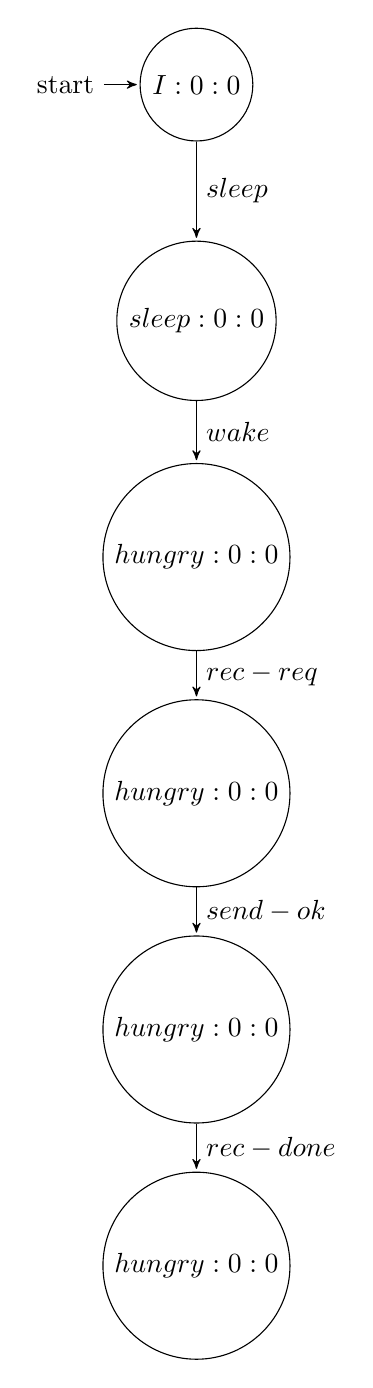
\begin{tikzpicture}[>=stealth',shorten >=1pt,auto, node distance=3cm]

    \node[initial,state] (I-0) {$I:0:0$};
    \node[state]    (asleep-0)  [below of=I-0] {$sleep:0:0$};
    \node[state]    (hungry-0-0)  [below of=asleep-0] {$hungry:0:0$};
    \node[state]    (hungry-0-1)  [below of=hungry-0-0] {$hungry:0:0$};
    \node[state]    (hungry-0-2)  [below of=hungry-0-1] {$hungry:0:0$};
    \node[state]    (hungry-0-3)  [below of=hungry-0-2] {$hungry:0:0$};

    \path[->] (I-0) edge node {$sleep$} (asleep-0);
    \path[->] (asleep-0) edge node {$wake$} (hungry-0-0);
    \path[->] (hungry-0-0) edge node {$rec-req$} (hungry-0-1);
    \path[->] (hungry-0-1) edge node {$send-ok$} (hungry-0-2);
    \path[->] (hungry-0-2) edge node {$rec-done$} (hungry-0-3);

\end{tikzpicture}
\end{minipage}
\begin{minipage}{.3\textwidth}
\begin{tikzpicture}[>=stealth',shorten >=.8pt,auto, node distance=3.0cm]

    \node[initial,state] (I-1) {$I:0:0$};
    \node[state]    (hungry-1-0)  [below of=I-1] {$hungry:0:0$};
    \node[state]    (hungry-1-1)  [below of=hungry-1-0] {$hungry:1:0$};
    \node[state]    (hungry-1-2)  [below of=hungry-1-1] {$hungry:2:0$};
    \node[state]    (hungry-1-3)  [below of=hungry-1-2] {$hungry:2:1$};
    \node[state]    (hungry-1-4)  [below of=hungry-1-3] {$hungry:2:2$};
    \node[state]    (eating-1-0)  [below of=hungry-1-4] {$eating:2:2$};
    \node[state]    (sleeping-1-0)  [below of=eating-1-0] {$sleep:0:0$};

    \path[->] (I-0) edge node {$wake$} (hungry-1-0);
    \path[->] (hungry-1-0) edge node {$send-req$} (hungry-1-1);
    \path[->] (hungry-1-1) edge node {$send-req$} (hungry-1-2);
    \path[->] (hungry-1-2) edge node {$rec-ok$} (hungry-1-3);
    \path[->] (hungry-1-3) edge node {$rec-ok$} (hungry-1-4);
    \path[->] (hungry-1-4) edge node {$eat$} (eating-1-0);
    \path[->] (eating-1-0) edge node {$sleep$} (sleeping-1-0);

\end{tikzpicture}
\end{minipage}
\begin{minipage}{.3\textwidth}
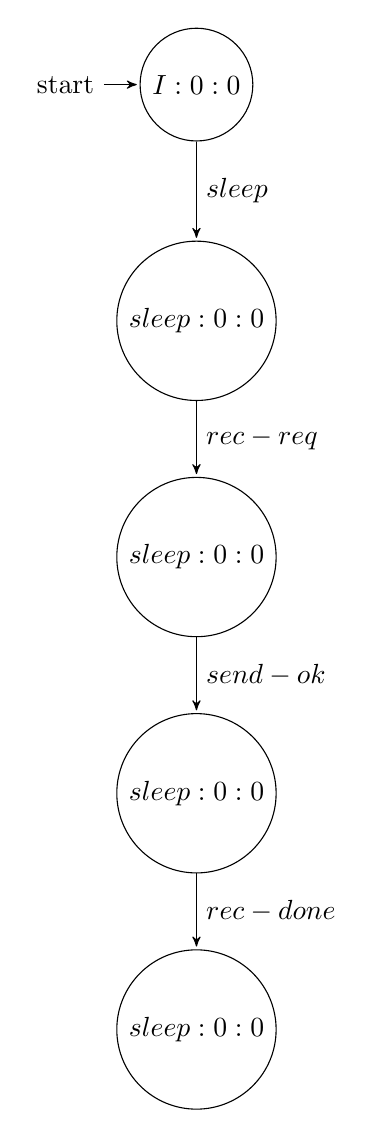
\begin{tikzpicture}[>=stealth',shorten >=1pt,auto, node distance=3cm]

    \node[initial,state] (I-0) {$I:0:0$};
    \node[state]    (asleep-2-0)  [below of=I-0] {$sleep:0:0$};
    \node[state]    (asleep-2-1)  [below of=asleep-2-0] {$sleep:0:0$};
    \node[state]    (asleep-2-2)  [below of=asleep-2-1] {$sleep:0:0$};
    \node[state]    (asleep-2-3)  [below of=asleep-2-2] {$sleep:0:0$};

    \path[->] (I-0) edge node {$sleep$} (asleep-2-0);
    \path[->] (asleep-2-0) edge node {$rec-req$} (asleep-2-1);
    \path[->] (asleep-2-1) edge node {$send-ok$} (asleep-2-2);
    \path[->] (asleep-2-2) edge node {$rec-done$} (asleep-2-3);


\end{tikzpicture}
\end{minipage}

    \caption{Dining philosopher traces. Each process maintians 3 state
    variables, [$currentState$,$OustandingRequests$,$AcksReceived$]. When hungry a
philosopher requests to eat from its neighbour, each request increases
outstandingRequets. A philosopher can eat after receiving two acks.}
\end{figure*}


\begin{figure*}
\begin{tikzpicture}[>=stealth',shorten >=.8pt,auto, node distance=4.0cm]

    \node[initial,state] (I-1) {$I:0:0$};

    %s1
    \node[state]    (hungry-1-0)  [below right of=I-1] {$hungry:0:0$};

    \node[state]    (hungry-1-1)  [below right of =hungry-1-0] {$hungry:1:0$};
    \node[state]    (hungry-1-2)  [below left of=hungry-1-1] {$hungry:2:0$};
    \node[state]    (hungry-1-3)  [above left of=hungry-1-2] {$hungry:2:1$};
    \node[state]    (sleeping-1-0)  [below left of=I-1] {$sleep:0:0$};
    \node[state]    (eating-1-0)  [below left of=sleeping-1-0] {$eating:2:2$};
    \node[state]    (hungry-1-4)  [below right of=eating-1-0] {$hungry:2:2$};

    \path[->] (I-0) edge [bend left ]node {$wake$} (hungry-1-0);
    \path[->] (I-0) edge [bend right] node {$sleep$} (sleeping-1-0);

    \path[->] (hungry-1-0) edge node {$send-req$} (hungry-1-1);
    \path[->] (hungry-1-1) edge node {$send-req$} (hungry-1-2);
    \path[->] (hungry-1-2) edge node {$rec-ok$} (hungry-1-3);
    \path[->] (hungry-1-3) edge node {$rec-ok$} (hungry-1-4);
    \path[->] (hungry-1-4) edge node {$eat$} (eating-1-0);
    \path[->] (eating-1-0) edge node {$sleep$} (sleeping-1-0);


    \path[->] (hungry-1-0) edge [loop left] node {$rec-req$} (hungry-1-0);
    \path[->] (hungry-1-0) edge [loop right,swap] node {$send-ok$} (hungry-1-0);
    \path[->] (hungry-1-0) edge [loop below] node {$rec-done$} (hungry-1-0);

    \path[->] (sleeping-1-0) edge [loop left] node {$rec-req$} (sleeping-1-0);
    \path[->] (sleeping-1-0) edge [loop right] node {$send-ok$} (sleeping-1-0);
    \path[->] (sleeping-1-0) edge [loop below] node {$rec-done$} (sleeping-1-0);

    \path[->] (sleeping-1-0) edge [bend right] node {$wake$} (hungry-1-0);

\end{tikzpicture}
\caption{Aggregate state machine from 3 traces, using exact state matching}
\end{figure*}

%\begin{adjustbox}
%\end{adjustbox}

\subsection{Invariant Detection, and operation inference}

Using exact state matching the FMS generated from the aggregation of traces is
a strict under representation of a systems behavior (\todo{find a fundamental
paper on dynamic analysis}), therefore all safety, and liveness violations are
correct. In practice exact state matching results in a massive FSM with few
inferred paths to traverse (as the likelihood of variables such as buffers,
id's and ports matching is low). Relaxed state matching generates a smaller FSM
with more paths to explore. However, matching on a subset of state allows
false positives in both safety, and liveness detection. Here we present a novel
technique for identifying safety and liveness conditions on relaxed state
matching which orders violations by their likelihood of being false positives.
This technique uses simulated values for variables which do not match, and
invariant violations as a heuristic measure of divergence from the real system.

Each node $n$ is composed of a set of matching states, $n =
{s_0,s_1,\dots,s_n}$. Some subset of variables in each matching state $s =
{v_0,v_1,\dots,v_m}$ match, while another subset of variables do not. The
subset of variables which do not match form a sub trace which profiles their
behavior. We use Daikon to detect data invariants which held during
execution~\cite{Ernst07}.

Edges connecting nodes are state transitions with an associated operation on
the state. In the case of \textbf{State Matching} transitions between state,
are equivalent to an assignment statement (ie if node $n$ and $n$ are
constructed from exactly matching states, for any transition $e$ between states
$\forall i$, $v_i == v'_i$. \textbf{Relaxed State Matching} is more
complicated, because many values may exist for any variable $v$ in state $n$. A
transition between two states may not be valid in the case of \textbf{Relaxed
State Matching}, as the aggregate state is an over approximation of the systems
observed behavior.

To reduce false positives when applying \textbf{Relaxed State Matching} the
values of unmatched variables are simulated during runtime. If the trace
produced by the runtime violates invariants detected from real executions, the
probability of a violation being a false positive increases \todo{this is a big
claim, and one that will need to be backed up. If it is true it will be a
research contribution.} To simulate variable values, we synthesize operations
using Z3, and input output examples from traces~\cite{SMTSynth}. The state
transitions inferred by Z3 are applied to variables during runtime. In cases
where no operations could be inferred within a given timeout, a value is
deterministicly chosen for relaxed variable.

\begin{figure*}
    \includegraphics[width=\textwidth]{fig/relaxed}
\end{figure*}


\subsection{Runtime}

\todo{Our} runtime executes replicated versions of the inferred state machine.
Each machine can send and receive messages to any other machine, and execute
local events. The number of state machines to execute is a user defined
parameter. More machines increase runtime, but may detect subtle bugs reliant
on complicated multi machine state. Algorithm ~\ref{alg:runtime} overview our
runtime engine.

\begin{algorithm}
    \caption{Runtime Algorithm}
    \label{alg:runtime}
    \KwData{$Replication, Depth, Model, Conditions$}
    \KwResult{Condition Violating Traces}
    \While{$Depth \geq 0$}{
        $eventQueue \gets GenEvents(Model,Replication)$ \\
        \While{$\neg eventQuene.Empty()$}{
            $ApplyEvent(eventQueue.Pop())$
            $CheckSafty(Conditions)$
            $CheckLiveness(Conditions)$
            $Recurse(Replication,Depth--,Model,Conditions)$
        }
    }
\end{algorithm}

Initial all machines are set to an empty initial state $\perp$. All valid events are
generated at the beginning of the main runtime loop. A valid event is the set
of all outgoing edges of all the current state of all nodes. Each event is
added to an event queue and is applied systematically. Three kinds of events can
be applied at runtime.

\begin{itemize}

    \item\emph{Local Event} A local event transitions a single node from one state to another.

    \item\emph{Send Event} A send event generates a message, which is placed on an outstanding message list

    \item\emph{Receive Event} A receive event consumes a message. Two conditions
        exist for receiving messages, droppable, and undroppable. Droppable
        message can be consumed by any machine in any state, if no transition
        exists for the message, the state of the received machine does not
        change. Undroppable messages are only delivered to machines which are in
        a state with a transition corresponding to the message being
        received~\cite{yang_modist_nsdi09}.

\end{itemize}


Messages are consumed by only a single node. As our search is performed
systematically, all permutations of message delivery are eventually explored. 

While executing a trace of variables is maintained. Variables are updated during
each state transition. If the state transitioned into is exactly matched,
runtime variables are assigned the value of the state. Otherwise the operations
determined by constraint solving are applied to the variables.

The runtime environment has a holistic view of the system, and is therefore
able to check safety predicates at all times. Predicates defined by a user
specification, such as only one machine may enter the critical section at a
time, or at least one node has a token, are checked on a per variable basis.

Liveness conditions are checked using techniques developed by
~\cite{Garg:2014:MAS:2580115.2580404}. If a periodic pattern is found in a
distributed execution, ie if at two points in an execution, the state of the
system is exactly the same, the events between the two states can periodically
execute forever (given non random liveness guarantees). If exact states are
revisited during runtime, and a liveness condition is not met over the interval
between matching states, a liveness violation is reported.

\subsection{Violations \& false positive reduction}

The result of simulating is a set of traces on which a safety or liveness
violation occurred. Traces contain vector time stamps for simulated events,
which are formatted to be visualized by ShiViz, to aid in
debugging~\cite{Abrahamson_sheddinglight}. Traces generated using \textbf{State
Matching} and \textbf{Event Matching} are guarantees bugs, the traces of which
can be traversed to identify the root cause of the bug. 

Traces generated using \textbf{Relaxed State Matching} and \textbf{Relaxed
Event Matching} may be false positives. These traces are approximately ordered by
their likelihood to be false positives. Each simulated trace (containing
simulated variable values at runtime) is analyzed by Daikon. Using Daikons
Invariant Difference tool the count of invariant violations generated by the
simulated execution can be determined. Traces which violate the minimum count
of invariants are reported to the user first, as they are least likely to have
diverged from the systems real behavior.



\input{evaluation}
\input{timeline}


\balance
\bibliographystyle{abbrv}
\bibliography{paper}

\end{document}
